\subsection{The Standard Model}

Before the protagonist
\footnote{Really the ensemble cast, given that they come in three flavors, electron($e\nu$), muon ($\mu \nu$) and tau($\tau \nu$)and their respective antiparticles,}
of our story - the neutrino - can be formally introduced, the stage has to be set.
A good candidate to set the stage would be the standard model which describesthree of the four known fundamental forces, electromagnetic, weak and strong interactions (it struggles to deal with  gravity) and classifying all known elementary particles.
Just like any foundational theory that undergirds a subfield of a subject, the standard model definitely wasn't developed in a day and as such, it may behoove us to at least go over the high points ofits development in order to have a better understanding of the context that surrounds neutrinos.

One may definitely quibble about where our understanding of the fundamental particles starts from, after all, humans have been trying to find out the nature of our universe and the things that make it up going back as far as the 4th century BCE with Plato positing that everything is made up of 4 elements (water, wind, earth and fire)\cite{Timaeus} but I think it makes sense to start at the discovery of the first of the particles that made it's way into the pantheon of the standard model; the electron.
For the longest time, humans had thought that atoms were the smallest particle that makes up everything in the world and cannot be subdivided further\cite{Dalton} but this idea had started to come under scrutiny by the late 1800's.
Even then, it was thought that if anything were to make up atoms, they would n't be lighter than the lightest atom.
However, in 1897, Thomson would come in with evidence that there not only were particles that made up the atoms, but that they were on the scale of 1000 times lighter  than hydrogen.
He decided to shoot cathode rays at a thermal junction so he could measure the generated heat and neasured how much they deflectedmagnetically.
He also measured the electrical deflections by lowering the pressure in the chamber where he was measuring the deflection.
Through these experiments, discovered the electron
\footnote{Although Thomson did decide to call them corpuscles; a name which definitely did not stick around}
and believed that it was a fundamental part of all atoms that was very light and held a decidedly negative charge.\cite{electronDiscovery}

The discovery of something so much smaller than the lightest atom threw Dalton's atomic theory out the window.
His theory claimed that  everything in the universe was made up of atoms which would vary in size and mass based on the element.
These atoms could not be created or destroyed, but  could reaarrange themselves through chemical reactions.
It could be argued that Dalton's model was a progenitor for the idea of conservation of mass and energy.
Despite being such an important idea, even before the discovery of electrons, the theory wasn't fullproof; it could not account for isotopes of the same element having different masses, but the electron blew the idea wide apart.

A new theory that looked at the atom not as the smallest thing that could exist but rather something that had other things inside in some sort of structure had to be developed.
There were numerous models that tried to tackle this problem and one of the first was proposed by Thompson in 1904 as the plum pudding model.
The first problem to grapple with was that electrons are negatively charged while the atoms themselves are electrically neutral.
To get around this, the plum pudding model suggests that  the electrons were suspended in a morass of positively charged particles
\footnote{Kind of like plums suspended in a pudding, hence the name of the model}
with the charge between the positive  and negative equalling out to 0.
Thomson believed that the mass was evenly distributed throughout the atom.

\begin{figure}[H]
  % https://en.m.wikipedia.org/wiki/File:Plum_pudding_atom.svg
  \centering
  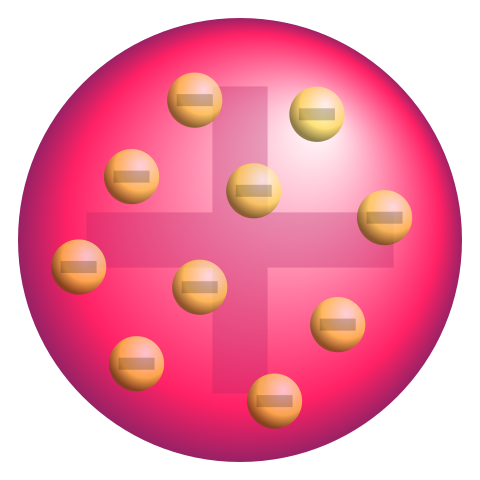
\includegraphics[width=100mm]{figures/plumPudding.png}
  \caption{Cartoon of plum pudding model}
  \label{plumPudding}
\end{figure}

The plum pudding model struggled to explain how these charged particles were so copacetic with each other despite being such small physical distances apart.
It was well known by then that opposite charges attract while alike charges repel.
It also failed to provide any explanation of the spectral lines observed in hydrogen.
Dark clouds were still on the horizon for Thomson's plum pudding model.
Between 1908 and  1913, a number of alpha ($\alpha$) particle scattering experiments were performed by Hans Geiger and Ernest Marsden.
These took the form of shooting $\alpha$  particles at a  incredibly thin piece of gold foil.
Based on the plum pudding model, it was expected that the $\alpha$ particles would not be deflected however this turned out not to be the case at all.
To be fair, most of the $\alpha$ particles did indeed go straight through the gold foil, their trajectory not disturbed in the slightest.
A smaller fraction did get deflected, some by a small angle and others by a large one.
But the astonishing part was that an even smaller fraction, about 1 in 20000, shot right back at the direction the particle gun was shooting from.

\begin{figure}[H]
   % https://en.wikipedia.org/wiki/Rutherford_scattering_experiments#/media/File:Geiger-Marsden_experiment_expectation_and_result.svg
  \centering
  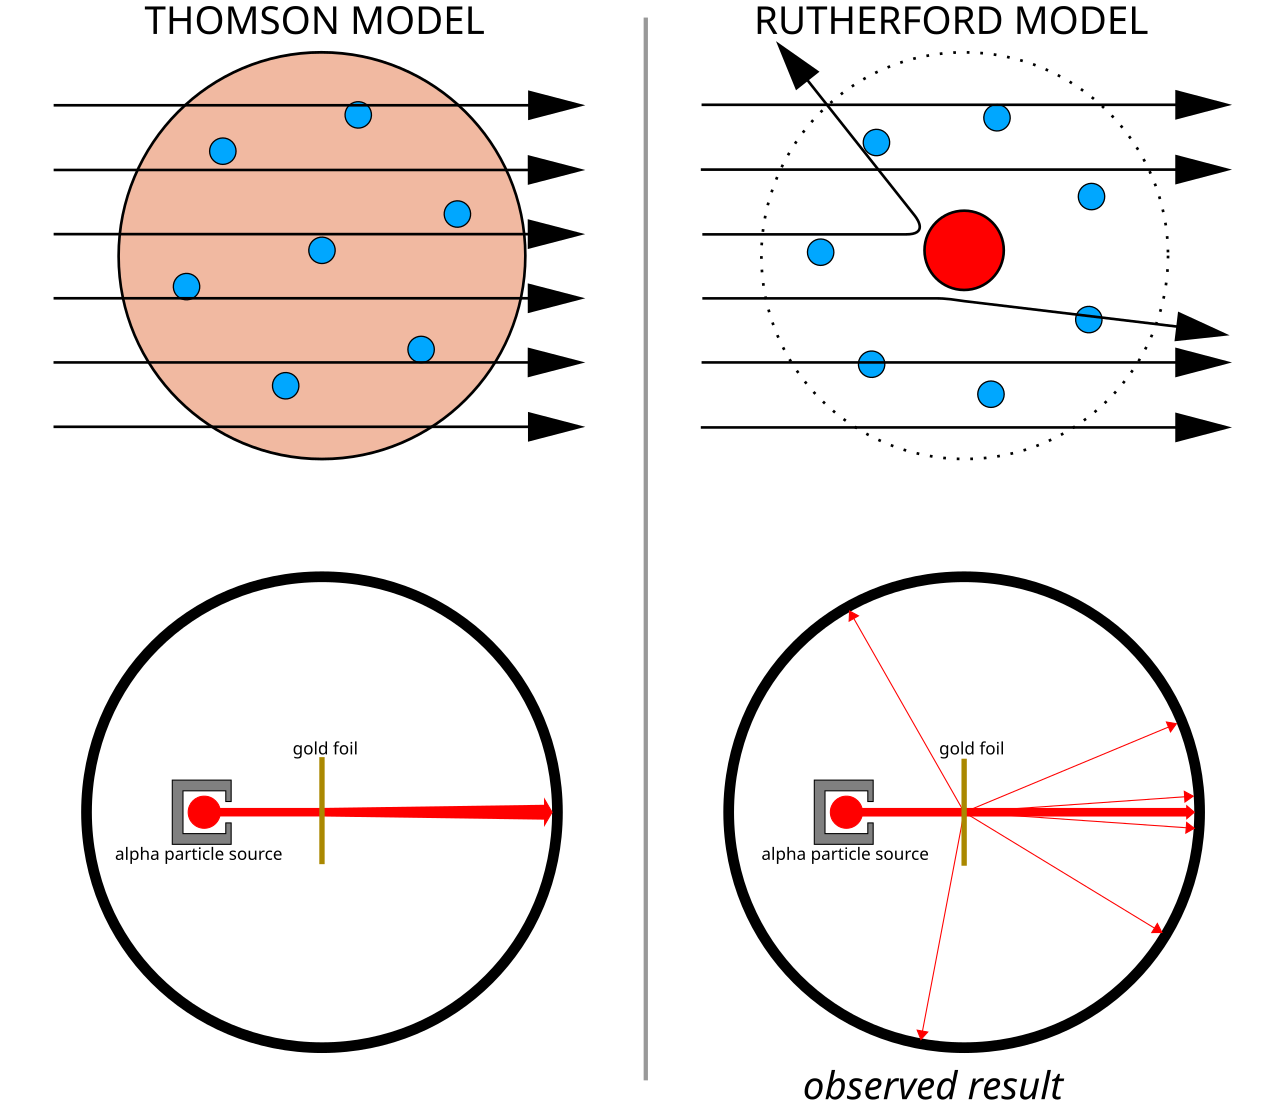
\includegraphics[width=100mm]{figures/goldFoil.png}
  \caption{Cartoon of Gold foil experiment}
  \label{goldFoil}
\end{figure}

So a new model was required to explain the discrepencies away; in comes Rutherford.




